\documentclass{article}
\usepackage[utf8]{inputenc}
\usepackage{hyperref}
\title{Demo Paper: Atomic Bonded Cross-chain Debt}
% \author{
%   \texttt{Amirhossein Khajehpour\samethanks}\\
%   amirhosseinkh@ce.sharif.edu
%   \and
%   \texttt{Fatemeh Bagheri\thanks{These authors contributed equally to this work.}}\\
%   fateme.bagheri95@student.sharif.edu
%   \and
%   \texttt{Melika Abdi}\\
%   melika.abdi@ee.sharif.edu
% }
\author{
  \texttt{Amirhossein Khajehpour\thanks{These authors contributed equally to this work.}}\\
  amirhosseinkh@ce.sharif.edu
  \and
  \texttt{Fatemeh Bagheri\samethanks}%\\
%   fateme.bagheri95@student.sharif.edu
  \and
  \texttt{Melika Abdi}\\
  melika.abdi@ee.sharif.edu
%   \and
%   \texttt{Melika Abdi\samethanks}\\
%   melika.abdi@ee.sharif.edu
}
\date{January 2021}

\usepackage{natbib}
\usepackage{graphicx}

\newcommand*\samethanks[1][\value{footnote}]{\footnotemark[#1]}

\begin{document}

\maketitle
\section{Abstract}
Atomic Bonded Cross-chain Debt (ABCD) is the first non-custodial smart-contract-independent cross-chain atomic bond. Theoretical aspects of ABCD have been presented in the ICBTA and won the best presentation award. It is the first time a demo of Atomic Bonded Cross-chain Debt is presented. 

\section{Introduction}
ABCD~\cite{tefagh2020atomic} is an atomic protocol used to exchange bonds. The seller of the bond gets some principal from the buyer, uses it for some trades, and repurchases it before a certain time. In this protocol, there is a secret on the bond buyer's principal so that the principal is not spendable until the secret is revealed by the buyer. Thus, the bond seller has to use the hash of this secret in all her trades. She can only exercise the trades when she pays her debt back and hence the buyer reveals the secret. The seller also pays an arbitrary amount to the buyer as a premium to incentivize him.

In this demo, Alice is the bond seller who borrows the principal and pays the premium, Bob is the bond buyer who lends the principal and gets the premium. Carol is the party with whom Alice makes another trade before paying Bob's principal back. Alice takes the principal from Bob in the Bitcoin testnet, performs an atomic swap with Carol between Bitcoin and Litecoin testnets, and pays Bob's principal back in Bitcoin. This is the normal way the protocol goes on. Of course, at any point, some coalition may decide to stop the procedure or intentionally deviate from the protocol in order to maximize their utility. The protocol supports situations where any set of parties behave abnormally. If Bob defaults, he will be punished by losing his margin. If either Alice or Carol defaults, Bob will gain the premium anyway. Finally, if Alice and Carol adhere to the protocol, and Bob avoids revealing the leader key, then Alice can punish Bob by acquiring Bob's guarantee amount. 

\begin{figure}
    \centering
    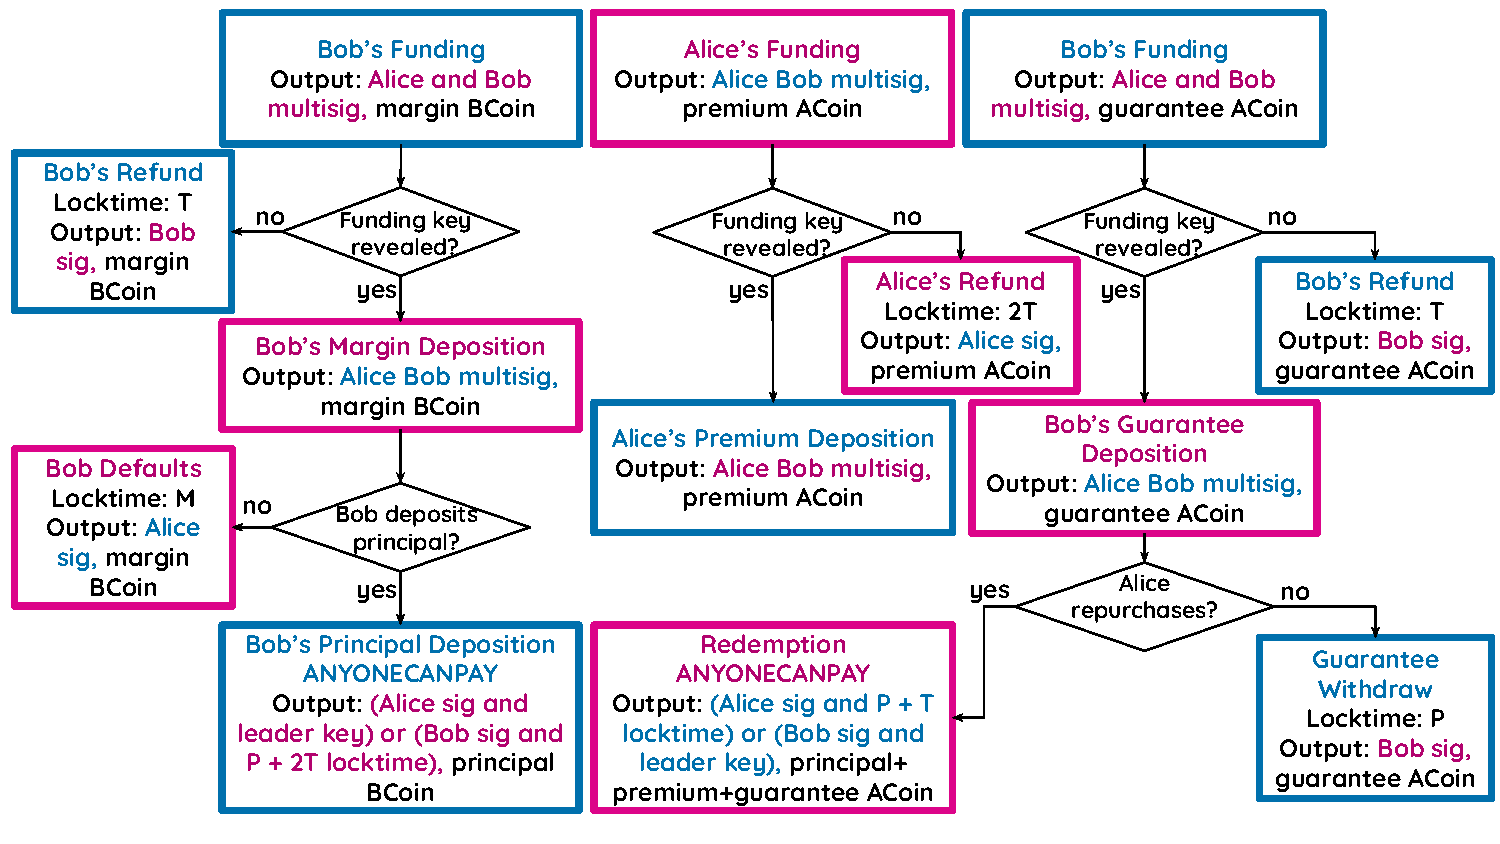
\includegraphics[width=\textwidth]{ABCDfateme.pdf}
    \caption{ A flowchart for the protocol. All the transactions and their output scrips are shown. }
    \label{fig:flowchart}
\end{figure}
% \hfill mds
 
% \hfill August 26, 2015
\section{Transactions}
Fig. \ref{fig:flowchart} shows the flow of the protocol and all the transactions. Transactions included in the ABCD are the followings:
\begin{itemize}
    \item Funding: There are three funding transactions, one for Alice and two for Bob. In order to spend the funding transactions, either the \textit{funding key} has to be revealed or a certain amount of time has to be passed. The former represents the normal case, while the latter happens if Alice does not reveal the key.
    \item Refund: In case of any abnormal action from the other party, each party can use the refund to take the funding amount back.
    \item Margin Deposition and Guarantee Deposition: Using these transactions Alice moves Bob's fundings amount to the next step and also reveals the funding key. After confirming margin deposition and guarantee deposition transactions, Bob's refund transactions no longer work.
    %mention earlier that this is why Bob does the whole thing
    \item Premium Deposition: When Alice reveals the funding key, Bob broadcasts this transaction to pay the premium to himself and both parties go to the next stage.
    \item Redemption: This transaction is used for Alice to repurchase the bond. This is an any-one-can-pay transaction which means at the time of creating, not all the inputs need to be clear. Alice can later fulfill the inputs and pay her debt back. 
    \item Bob's Principal Deposition: Bob has to broadcast this transaction before $M$ locktime. By doing this, he is lending the principal to Alice. This transaction can not be spent without knowing the \textit{leader key}. So, Bob does not reveal it until Alice has broadcast the redemption.
    % \item Alice Defaults: If Alice does not pay her debt back before $P$ locktime, Bob will broadcast this transaction and get his premium. He will never reveal the leader key so that Alice can not spend the bond.
    \item Bob Defaults: If Bob does not deposit the principal before $M$ locktime, Alice will take his margin as a punishment using this transaction.
    \item Guarantee Withdrawal: If Alice repurchases the bond within the expected time and Bob does not reveal the leader key, then Alice can punish Bob by spending the guarantee amount on the repurchase transaction to herself. Otherwise, Bob can pay the guarantee value back to himself using the guarantee withdrawal transaction.
\end{itemize}


\section{Protocol}
The protocol of ABCD consists of two phases, initialization, and commitment.\\
\textbf{Initialization Phase}:
In this phase, the parties create transactions, exchange, and sign them. So, they make sure no one has the chance to cheat on the other. Fig.~\ref{fig:initialization} is an illustration of this phase. Steps of this phase are:
\begin{enumerate}
    \item Alice creates the funding and refund transactions and sends them to Bob. Then, Bob signs the refund and sends it back to Alice. Now, Alice signs the funding and refund transactions. Bob does likewise to Alice. 
    \item Alice creates the margin deposition and guarantee deposition transactions and sends them to Bob. Bob signs them and sends them back to Alice. Then Alice signs and keeps them. Bob does likewise for the guarantee withdrawal transaction and then for the premium and principal deposition transactions. Then, Alice does the same for the redemption transaction.
    \item Finally, Alice shows the principal deposition transaction to Carol. Then, Carol creates an HTLC between herself and Bob.
\end{enumerate}
\begin{figure}
    \centering
    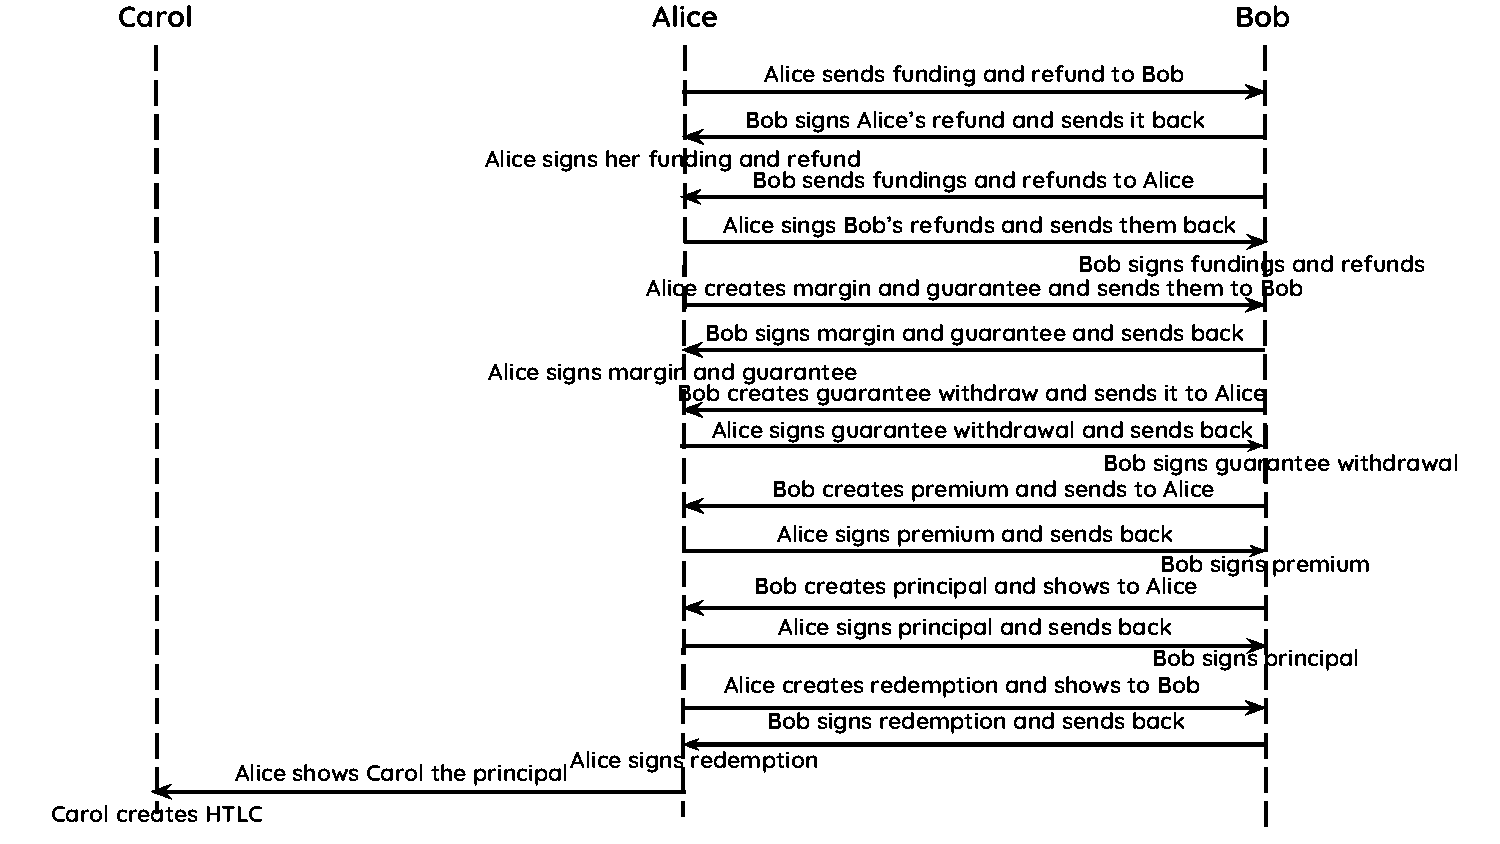
\includegraphics[width=\textwidth]{ABCDinitialization.pdf}
    \caption{Initialization phase}
    \label{fig:initialization}
\end{figure}
\textbf{Commitment Phase:}
In this phase, they broadcast the transactions created in the last phase dependent on whether they wish to abort everything or continue normally. Fig.~\ref{fig:commitment} is an illustration of this phase. The normal case can be divided into the following steps:
\begin{enumerate}
    \item Alice broadcasts the funding transaction. If she was willing to abolish the whole procedure, she would not broadcast the funding.
    \item Bob broadcasts his own fundings.
    \item Alice broadcasts the margin deposition and guarantee deposition transactions and reveals the funding key, so the funding key reveals to Bob. In the abnormal case, she would broadcast the refund and Bob would do likewise.
    \item Bob broadcasts the premium deposition transaction. If he does not, Alice will broadcast the refund. 
    %change the figure three
    \item Bob fulfills the principal deposition transaction and broadcasts it. In the case of Bob defaulting, he would not deposit the principal before the $M$ locktime. Therefore, Alice, broadcasting the Bob defaults transaction, would take his margin. %define default
    
    \item When Carol sees the principal deposition transaction, she broadcasts her HTLC. %If she does not, Alice defaults as well. % what happens exactly?
    \item Alice fulfills the redemption and broadcasts it. If she does not do it before the $P$ locktime, Bob would take his margin and guarantee back and he would not reveal the leader key.
    \item Bob spends the redemption. Doing this, he reveals the leader key.
    \item Now, Alice knows the leader key. Thus, she spends Carol's HTLC.
    \item Carol who now knows the leader key, spends Bob's principal and the procedure is over.
\end{enumerate}

% \subsection{Subsection Heading Here}
% Subsection text here.


% \subsubsection{Subsubsection Heading Here}
% Subsubsection text here.


% An example of a floating figure using the graphicx package.
% Note that \label must occur AFTER (or within) \caption.
% For figures, \caption should occur after the \includegraphics.
% Note that IEEEtran v1.7 and later has special internal code that
% is designed to preserve the operation of \label within \caption
% even when the captionsoff option is in effect. However, because
% of issues like this, it may be the safest practice to put all your
% \label just after \caption rather than within \caption{}.
%
% Reminder: the "draftcls" or "draftclsnofoot", not "draft", class
% option should be used if it is desired that the figures are to be
% displayed while in draft mode.
%
%\begin{figure}[!t]
%\centering
%\includegraphics[width=2.5in]{myfigure}
% where an .eps filename suffix will be assumed under latex, 
% and a .pdf suffix will be assumed for pdflatex; or what has been declared
% via \DeclareGraphicsExtensions.
%\caption{Simulation results for the network.}
%\label{fig_sim}
%\end{figure}

% Note that the IEEE typically puts floats only at the top, even when this
% results in a large percentage of a column being occupied by floats.


% An example of a double column floating figure using two subfigures.
% (The subfig.sty package must be loaded for this to work.)
% The subfigure \label commands are set within each subfloat command,
% and the \label for the overall figure must come after \caption.
% \hfil is used as a separator to get equal spacing.
% Watch out that the combined width of all the subfigures on a 
% line do not exceed the text width or a line break will occur.
%
%\begin{figure*}[!t]
%\centering
%\subfloat[Case I]{\includegraphics[width=2.5in]{box}%
%\label{fig_first_case}}
%\hfil
%\subfloat[Case II]{\includegraphics[width=2.5in]{box}%
%\label{fig_second_case}}
%\caption{Simulation results for the network.}
%\label{fig_sim}
%\end{figure*}
%
% Note that often IEEE papers with subfigures do not employ subfigure
% captions (using the optional argument to \subfloat[]), but instead will
% reference/describe all of them (a), (b), etc., within the main caption.
% Be aware that for subfig.sty to generate the (a), (b), etc., subfigure
% labels, the optional argument to \subfloat must be present. If a
% subcaption is not desired, just leave its contents blank,
% e.g., \subfloat[].


% An example of a floating table. Note that, for IEEE style tables, the
% \caption command should come BEFORE the table and, given that table
% captions serve much like titles, are usually capitalized except for words
% such as a, an, and, as, at, but, by, for, in, nor, of, on, or, the, to
% and up, which are usually not capitalized unless they are the first or
% last word of the caption. Table text will default to \footnotesize as
% the IEEE normally uses this smaller font for tables.
% The \label must come after \caption as always.
%
%\begin{table}[!t]
%% increase table row spacing, adjust to taste
%\renewcommand{\arraystretch}{1.3}
% if using array.sty, it might be a good idea to tweak the value of
% \extrarowheight as needed to properly center the text within the cells
%\caption{An Example of a Table}
%\label{table_example}
%\centering
%% Some packages, such as MDW tools, offer better commands for making tables
%% than the plain LaTeX2e tabular which is used here.
%\begin{tabular}{|c||c|}
%\hline
%One & Two\\
%\hline
%Three & Four\\
%\hline
%\end{tabular}
%\end{table}


% Note that the IEEE does not put floats in the very first column
% - or typically anywhere on the first page for that matter. Also,
% in-text middle ("here") positioning is typically not used, but it
% is allowed and encouraged for Computer Society conferences (but
% not Computer Society journals). Most IEEE journals/conferences use
% top floats exclusively. 
% Note that, LaTeX2e, unlike IEEE journals/conferences, places
% footnotes above bottom floats. This can be corrected via the
% \fnbelowfloat command of the stfloats package.



\section{Conclusion}

In this article, we run an instance of ABCD on Bitcoin testnet and perform a simple atomic swap with the debt and Litecoin testnet tokens. The reference to the implementation of different scenarios of ABCD is accessible in ABCD official github page \href{https://github.com/incentivus/abcd}{https://github.com/incentivus/abcd}.

\bibliographystyle{plain}
\bibliography{references}
\end{document}
